\documentclass[12pt]{article}
\usepackage[usenames,dvipsnames]{color}
\usepackage{listings}
\usepackage{graphicx}
\usepackage{fancyhdr}
\usepackage{framed}
\usepackage[T1]{fontenc}
\usepackage[toc,page]{appendix}
\usepackage[utf8]{inputenc}
\usepackage[brazil]{babel}
\usepackage{fancyvrb}
\usepackage[hmargin=2cm,vmargin=2cm]{geometry}
\usepackage{lastpage}
\usepackage{pdfpages}
\usepackage{makeidx}
\usepackage{hyperref}
\pagestyle{fancy}
\usepackage{enumitem}
% cabecalho e rodapé
\setlength{\headheight}{120pt}
\setlength{\textheight}{550pt}
\renewcommand{\headrulewidth}{0pt}
\lhead{
\includegraphics[scale=0.03]{brasao.png}}
%\chead{\includegraphics[scale=0.5]{logo-brasil-sem-pobreza2.png}}
\rhead{
\includegraphics[scale=0.5]{logo-pnud.png}}
\cfoot{\textbf{\ProjectCode\ - Inovando a democracia participativa}}
\rfoot{\thepage}

\hyphenation{par-ti-ci-pa-ção}
\bibliographystyle{ieeetr}

% definições sobre o autor e o produto
\newcommand{\MyName}{Renato Fabbri}
\newcommand{\MySurnameForename}{Fabbri, Renato}
\newcommand{\SupervisorName}{Gabriella Vieira Oliveira Gonçalves}
\newcommand{\MyEmail}{renato.fabbri@gmail.com}
\newcommand{\ContractNumber}{2013/000566}
\newcommand{\ContractYear}{2014}
\newcommand{\ProjectCode}{Projeto BRA/12/018}
\newcommand{\NomeSecretaria}{Secretaria-Geral da Presidência da República}
%Q\newcommand{\SiglaSecretaria}{SG/PR}
\newcommand{\SiglaSecretaria}{Secretaria: SNAS }
\newcommand{\ProductNumber}{04}
\newcommand{\ProductTitle}{Proposta de adaptações e incrementos para a interface do portal federal de participação social e suas ferramentas}
\newcommand{\ProductSubtitle}{com elementos visuais e de usabilidade para mecanismos de priorização de conteúdos e autorregulação}
\newcommand{\ProductDescription}{"Proposta de adaptações e incrementos para a interface do portal federal de participação sociais e suas ferramentas, com elementos visuais e de usabilidade para mecanismos de priorização de conteúdos e auto-regulação"}

\newcommand{\ProductValue}{R\$ 21,600 (vinte e um mil e seiscentos reais)}
\newcommand{\ObjetoContratacao}{
Aporte de conhecimentos e tecnologias para especificação de vocabulário e ferramentas assistidas que utilizam processamento de linguagem natural e análise de redes complexas para o conteúdo do portal da participação social.
}
\newcommand{\DataEntrega}{08 de Setembro de 2014}
\newcommand{\PalavrasChave}{reconhecimento de padrões, redes complexas, processamento de linguagem natural, participação social}

% lista de abreviações
\makeindex

\begin{document}


\newgeometry{hmargin=3cm,vmargin=1.5cm}
\begin{center}
\thispagestyle{empty}
{\color{MidnightBlue}


\includegraphics[scale=0.9]{logo-pnud.png}

\vspace{4cm}

{\bf \large \ProjectCode\ - Desenvolvimento de Metodologias
de Articulação e Gestão de Políticas Públicas para Promoção da Democracia
Participativa}

\vspace{1.5cm}

{\bf \large Produto \ProductNumber\ -\ \ProductTitle}

\vspace{1.5cm}

\ProductSubtitle

\vspace{4cm}

\MyName

\vspace{1cm}

}


\includegraphics[scale=0.04]{brasao.png} \\
{\bf \small \NomeSecretaria}

\end{center}
\restoregeometry
\newpage

\newgeometry{hmargin=3cm,vmargin=1.5cm}
\addtolength{\topmargin}{2.5cm}
\thispagestyle{empty}
{\color{MidnightBlue}

{\bf \LARGE Produto \ProductNumber\ -\ \ProductTitle}

\hrulefill

\vspace{1cm}

\begin{center}

{\bf \large Contrato n. \ContractNumber}

\vspace{1.5cm}

{\bf \large Objeto da contratação: \ObjetoContratacao}

\end{center}

\vspace{3.2cm}

Valor do produto: \ProductValue

\vspace{1.2cm}

Data de entrega: \DataEntrega

\vspace{1.2cm}

Nome do consultor: \MyName

\vspace{1.2cm}

Nome da supervisora: \SupervisorName

}

\vspace{2cm}

\begin{center}

\includegraphics[scale=0.04]{brasao.png} \\
{\bf \small \NomeSecretaria}
\end{center}

\restoregeometry
\newpage

\newgeometry{hmargin=3cm,vmargin=1.5cm}
\addtolength{\topmargin}{5cm}
\thispagestyle{empty}

\begin{framed}

{\raggedright \MySurnameForename} \\

\ProductTitle: \ProductSubtitle\ / \ContractYear. \\

Total de folhas: \pageref{LastPage} \\

\vspace{1cm}

Supervisor(a): \SupervisorName \\

\SiglaSecretaria \\

\NomeSecretaria \\

Palavras-chave: \PalavrasChave. \\

\end{framed}

\vspace{3cm}

{\raggedright 
\includegraphics{licenca-cc-by-nc.png} \ Esta obra é licenciada sob
uma licença Creative Commons - Atribuição-NãoComercial. 4.0 Internacional.}

\restoregeometry
\newpage

\tableofcontents
\newpage


\begin{abstract}
Este documento descreve rotinas de priorização de conteúdo e de autorregulação para o portal federal de participação social. Como parte da exposição e do Produto, foi implementado um sistema de recomendação de participantes para outros participantes e linha editorial do participa.br. Este sistema está online e visa atender a requisitos como os do ActionItem 3234 do Noosfero, que prevê recomendação de participantes, comunidades e empreendimentos. Como generalização da proposta, é delineada  recomendação de recursos como trilhas, artigos, comentários e palavras. O consultor e equipe do participa.br entendem que a disponibilização destes recursos em formato aberto - e com documentações reativas para fácil geração de derivados, críticas e propostas - é instrumental para a democracia participativa e online, promovendo empoderamento e transparência.\\

{\bf Palavras-chave:} \PalavrasChave.
\end{abstract}
\newpage

\section{Introdução}
\subsection{Contexto e importância da consultoria}
Em confluência com o portal federal de participação social (Participa.br) e o Plano Nacinal de Participação Social (PNPS), esta consultoria é um aporte de conhecimentos e tecnologias de web semântica, redes complexas e processamento de linguagem natural. O presente produto apresenta ``formas de priorização de conteúdo e de autorregulação'' na forma de um sistema de recomendação de recursos para participantes e linha editorial. No começo da seção~\ref{sec:dev} está explicitada a motivação para a implementação e a relação com o cumprimento dos termos deste Produto~\cite{termoReferencia}.

\subsection{Contexto e importância do Produto}
\subsubsection{Objetivos}
Este produto tem por objetivo principal a disponibilização de um sistema de recomendação de recursos do participa.br para usuários, tanto via critérios personalizados quanto considerando comunidades e linha editorial. Através deste sistema de recomendação, ficam facilitados, até mesmo prontamente disponíveis, diversos processos de autorregulação, de geração de resumos, de geração de relatórios e de análises informativas. Objetivos secundários são:
\begin{itemize}
    \item Disponibilização de uma API HTTP, para uso no participa.br, conforme requisitado pela equipe do Participa.br em diversos itens dos produtos~\cite{prodExtra}.
    \item A exposição destes algoritmos de recomendação aos visitantes web via uso de browsers comuns, para edição e execução dos trechos de código utilizados pela plataforma federal de participação social. Este objetivo foi satisfeito usando o IPython Notebook levantado para este trabalho~\cite{iNotebook}.
    \item Aproveitamento do endpoint SparQL com os dados do participa.br, fortalecendo as tecnologias de dados linkados e web 3.0~\cite{endpoint}.
    \item Em reunião com a consultora Daniela Feitosa, foi delineada a pertinência de um sistema de recomendação de perfis para um ActionIntem em andamento para o participa.br~\cite{actionItem}. Este produto visa suprir esta necessidade através da API disponibilizada para recomendações.
    \item A entrega das tecnologias livres com simplicidade e boa documentação, favorecendo o aproveitamento deste trabalho para melhoras, geração de derivados e novas e independentes tecnologias. Isso pode ser observado no repositório git público deste produto~\cite{repoProd4}.
    \item Compatibilizar ao máximo a entrega deste produto às demandas da equipe do participa.br~\cite{prodExtra}.
    \item Realizar de forma precisa e pertinente a especificação deste quarto produto no Termo de Referência~\cite{termoReferencia}.
\end{itemize}

\subsubsection{Resultados esperados}
De imediato e mais central, o resultado do produto é iniciar um processo aberto de desenvolvimento e apropriação de análises e mecanismos de autorregulação para o portal federal de participação social.

Como resultados diretos deste Produto, constam:
\begin{itemize}
    \item a habilitação para uso da API HTTP para recomendação de recursos do participa.br. Veja Apêndice~\ref{sec:api},~\ref{sec:infra} e~\ref{sec:inst}.
    \item A interface para apreensão e inovação dos algoritmos, não somente exemplificada ou projetada, mas operante e disponível. Veja Apêndice~\ref{sec:algs}.
    \item Um plano de implementação para o participa.br, que utiliza a API de recomendação para priorização de conteúdo e autorregulação. Veja Apêndice~\ref{sec:acr}.
    \item Transparência absoluta no trabalho, com toda a documentação e código computacional online em um repositório git que contem o histórico de implementação~\cite{repoProd4}.
    \item Algoritmos implementados em código de simples leitura, para facilitar a implementação em outras linguagens como Ruby ou Javascript, quando houverem recursos mais maduros para estas linguagens ou por necessidade. No momento, Python possui mais e mais maduros recursos tanto para redes complexas quanto para processamento de linguagem natural.
    \item Habilitação de implementações em andamento, como o plugin de recomendação de perfis~\cite{actionItem}, para recomendar amigos para participantes. 
\end{itemize}
\subsubsection{Caráter inovador}
Centralmente, este trabalho é inovador na aplicação de recursos de análise de redes sociais para empoderamento da sociedade civil, entregando as tecnologias e priorizando a reutilização. Este recurso é de vital interesse para a democracia participativa no contexto atual, com as revoluções da internet e das redes sociais. Permite, em última instância, que haja uma inteligência para aproveitamento das estruturas sociais, e que esta inteligência seja pública, transparente, minimizando vetores vigilantistas ou turvos.

Há a inovação na arquitetura em software, apresentando traços de web 3.0 como os dados linkados como base de conhecimento e os múltiplos recursos online acessados no funcionamento usual (ao menos Endpoint SparQL para acesso aos dados, API HTTP Flask para tratar os dados e gerar estatísticas e estruturas de interesse, Participa.br para interface e contexto pertinente).

Há inovação na difusão científica. Além dos métodos e tecnologias disponibilizadas, por exemplo, os termos Web Semântica, Processamento de Linguagem Natural e Redes Complexas são empregados em textos científicos e consistem em áreas que recebem pesquisas, revistas e até carreiras científicas inteiras. Neste Produto, este conteúdo está apresentado em português e se presta a facilitar contribuições de outras partes interessadas.

Os métodos de recomendação em si não foram confrontados exaustivamente com a literatura, mas possivelmente possuem também inovações nos procedimentos. Certamente há inovação no contexto de implementação, tanto de relevância social (portal federal de participação social) quanto de aparato tecnológico (web 3.0, métodos da física e de mineração de dados).

\subsubsection{Aparato em software e hardware}\label{subsec:hs}


O sistema de recomendação precisa ser mantido online, e isso implica na manutenção de uma estrutura em hardware e software que extrapola o objeto deste produto. As especificações desta arquitetura de software e hardware estão em um documento escrito pelo consultor a pedido da PR para a SNAS e DITEC~\cite{smDITEC}. Para fins de pesquisa e de entrega deste produto, o esquema da Figura~\ref{fig:sr} é realizado em máquinas de pesquisa da USP, concedidas para a pesquisa de doutorado do consultor. Tal configuração é razoável pois a pesquisa conflui e é potencializada por esta consultoria, mas está prevista uma infraestrutura própria da PR para estes serviços. Além disso, os usos atuais ainda são moderados, sem causar sobrecarga ao serviços de computação em nuvem da USP.

\begin{figure}[h!]
  \centering
      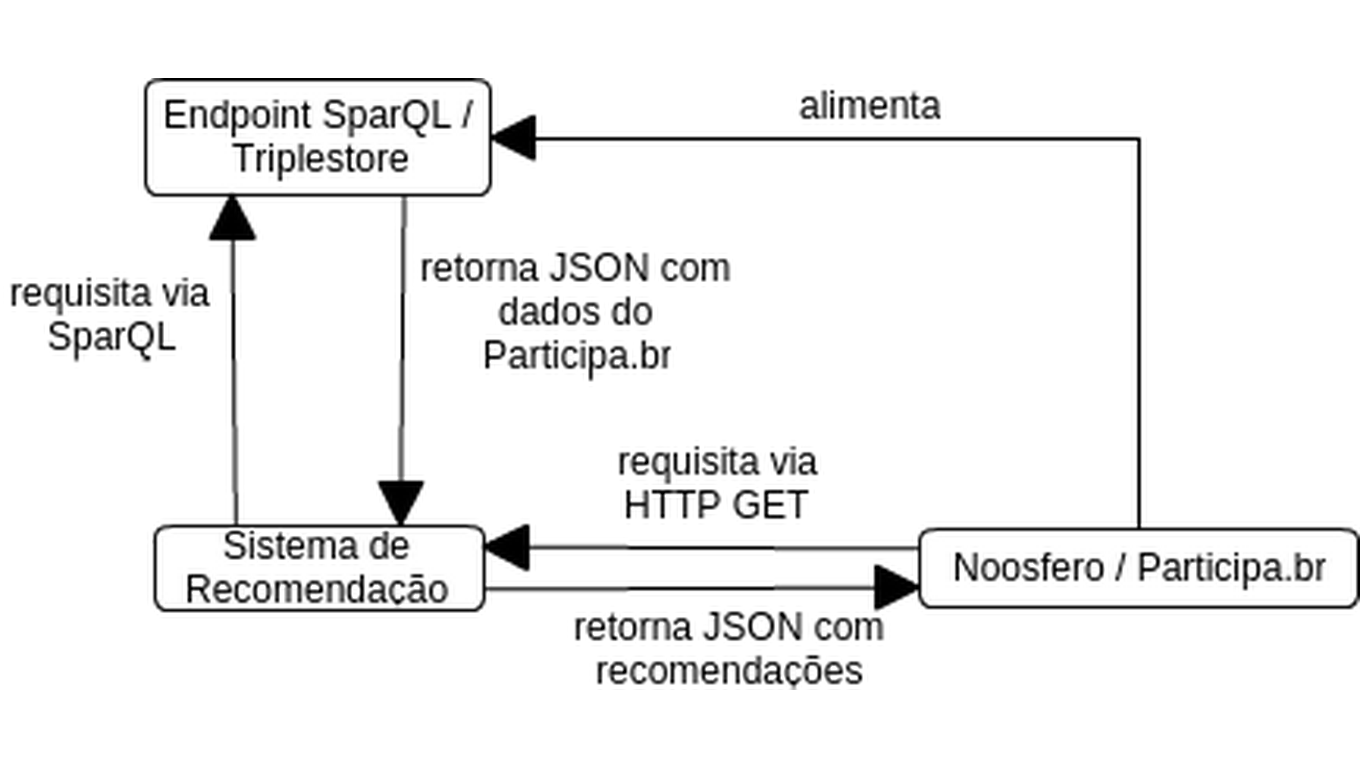
\includegraphics[width=0.8\textwidth]{sr}
  \caption{O sistema de recomendação e relações principais: com o frontend Participa.br e com a base de dados enriquecidos semanticamente.}\label{fig:sr}
\end{figure}

\section{Desenvolvimento}\label{sec:dev}
O produto é descrito no Termo de Referência desta consultoria assim: ``Documento com proposta de adaptações e incrementos para a interface do portal e suas ferramentas que inclua elementos visuais e de usabilidade para mecanismos de priorização de conteúdos e auto-regulação com base nos metadados gerados nativamente pela plataforma do portal e nas análises de PLN e RC produzidas pelas ferramentas assistidas''.

Dada a dimensão do participa.br, tanto da estrutura em software e das práticas participativas, quanto de mobilização humana, as propostas de adaptações para o portal são muitas e estão em diversos produtos deste e de outros consultores. Uma forma especialmente pertinente de realizar este produto, confluente com o Termo de Referência desta consultoria, com o trabalho dos gestores e comunidade e com os produtos deste e de outros consultores~\cite{prodExtra}, é a entrega de um sistema de recomendação de recursos para o participa.br.

Conforme discutido em reunião com gestores e comunidade do participa.br~\cite{padProd4}, em termos de \emph{priorização de conteúdo}, quase todos os casos de interesse para o atual participa.br podem ser considerados rotinas de recomendação. Além disso, dadas as práticas atuais de redes sociais, os mecanismos de autorregulação do participa.br são e serão baseados na adição de conteúdo por espontaneidade dos participantes. Esta dinâmica de adição espontânea de conteúdo pelos participantes conflui com sistemas de recomendação de recursos, pois estes podem catalizar sem coerção os processos participativos.

Desta forma, foi idealizada a entrega de um sistema de recomendação de recursos do participa.br para seus usuários, comunidades e linha editorial. As subseções a seguir apontam etapas na construção do sistema de recomendação. Os Apêndices~\ref{sec:api} e~\ref{sec:algs} concentram aspectos de operação do sistema. Os Apêndices~\ref{sec:infra} e~\ref{sec:inst} são voltados para os componentes e a instalação da versão operante deste sistema de recomendação de recursos. A seção~\ref{sec:uso} e o Apêndice~\ref{sec:acr} apreendem previsões e propostas de integração com o participa.br.

\subsection{Etapas de desenvolvimento anteriores a este produto}
\subsubsection{Sistematização ontológica da participação online}
Através de estudos e reuniões presenciais e online, a Ontologia de Participação Social (OPS) foi revisada~\cite{OPS} e a Ontologia do Participa.br (OPA) foi feita~\cite{OPA}.
\subsubsection{Triplificação dos dados do participa.br}
Feito um script para triplificar os dados do Participa.br, ou seja, para o enriquecimento semântico e escrita em RDF dos dados em Postgresql da instância Noosfero do Participa.br~\cite{triplifica}.
\subsubsection{Levantamento do endpoint SparQL}
Para uso dos dados triplificados, pode-se recorrer a diversos métodos de leitura e disponibilização. Um método-chave é a disponibilização dos dados rdf (\emph{triple store}) em um \emph{endpoint sparql}. Para os fins de testes, pesquisa e usos leves, está disponibilizado um endpoint SparQL em servidores da USP~\cite{endpoint}.
\subsubsection{Análises iniciais, modelos}
Análises dos dados do participa.br foram abertas no IPython Notebook, com ênfase no texto produzido e nas redes formadas~\cite{repoProd3}.
\subsection{Etapas de desenvolvimento deste produto}
\subsubsection{Reuniões com equipe do participa.br}
Especial agradecimentos ao Ricardo Poppi, Ronald Costa, Enaile Ladanza, Joênio Costa, Daniela Feitosa e Fernando Cruz.
\subsubsection{Estudos de aprofundamento e amadurecimento}
Em especial, foram lidos todos os produtos entregues pelos consultores, (re)visitados cursos no coursera e literatura científica~\cite{prodExtra}.
\subsubsection{Escrita deste documento}
Através da escrita deste documento, várias informações foram organizadas e sistematizadas, facilitando compreensão do contexto para especificação da API de recomendação e entrega do produto.
\subsubsection{Especificação da API de recomendação}
Basicamente, é convencionado um padrão na montagem das URLs para recomendar recursos de tipos especificados, para destinatários e por métodos também especificados. O Apêndice~\ref{sec:api} é dedicado a expor a convenção inicial entre URLs formadas e as recomendações que retornam.
\subsubsection{Implementação do serviço para aquisição dos dados, processamento e entrega em JSON}
Para a API da etapa acima, foi necessário desenvolver um servidor HTTP simples (em Flask). Veja pasta flask/ de~\cite{repoProd4}. 
\subsubsection{Disponibilização das rotinas no IPython Notebook}
Para expor os critérios de recomendação, disponibilizar análises e facilitar novas versões para as recomendações, as rotinas estão em um IPython Notebook. Veja o Apêndice~\ref{sec:algs} para uma exposição e detalhamento destas rotinas.
\subsubsection{Proposta de implementações no portal federal de participação social}
Com base no sistema de recomendações, nas demandas levantadas em reuniões e nos produtos já feitos por este e outros consultores, foi sistematizado um conjunto de propostas de acréscimos para o portal federal, detalhado no Apêndice~\ref{sec:acr}.
\subsection{Justificativa do método}
São usados diversos métodos neste produto. As justificativas se concentram nas tecnologias de web 3.0 (dados linkados e computação em nuvem), nas técnicas mais fundamentais/básicas/simples e nas demandas da equipe do participa.br, observadas através de reuniões e documentações produzidas recentemente pela equipe~\cite{prodExtra}.
\subsection{Justificativa das fontes}
A equipe do participa.br é uma equipe estratégica da Presidência da República voltada para participação social. As fontes externas utilizadas, como artigos, livros e videos, são garimpadas como atual pesquisa acadêmica principal do consultor.
\subsection{Confronto entre os resultados esperados e os alcançados}
No Termo de Referência desta consultoria, este produto é descrito como ``Documento com proposta de adaptações e incrementos para a interface do portal''. Este produto entrega estas propostas a serem implementadas no portal federal de participação social. Além disso, para facilitar estas implementações e fazer a conexão com os desenvolvimentos ontológicos e de dados linkados, foi implementado e disponibilizado um sistema de recomendação de recursos para o participa.br. Um outro resultado para além do esperado, é a consideração cuidadosa da comunidade de democracia participativa, com a disponibilização das rotinas de recomendação no IPython Notebook~\cite{iNotebook} e uma visita aos produtos dos outros consultores~\cite{prodExtra}.

\section{Usos dos resultados}\label{sec:uso}
Há usos previstos do sistema de recomendação, pois são demandas da equipe que motivaram o seu desenvolvimento. Em especial, há o uso previsto no plugin de recomendação de perfis (ActionItem~\cite{actionItem}).

Há usos próprios dos participantes, como consultas aos recursos recomendados para si e para outros, e usos para a linha editorial do portal. Estes usos podem ser feitos no próprio servidor que disponibiliza o serviço de recomendação. Podem ser adaptados para a interface do participa.br, com plugins ou temas apropriados. Algumas sugestões de implementações estão no Apêndice~\ref{sec:acr}.

Outro uso previsto, e que idealmente contará com incentivos da comunidade, é a evolução destes métodos de recomendação de perfis para melhor atender aos usos do portal e das comunidades. O consultor sugere que as comunidades sejam convidadas a apresentar uma ou mais pessoas com conhecimentos ou diposição para algoritmos e sistematizações. Esta pessoa poderia passar, por exemplo, por uma reunião para apreensão dos métodos de recomendação e análise, com vistas a proposição de melhoras e ampliação das funcionalidades.

As rotinas de recomendação estarão disponíveis online, e editáveis e executáveis no browser via IPython Notebook, o que deve facilitar dinâmicas de compartilhamento e amadurecumento destes processos. Este uso dos resultados deste produto é ainda mais central do que a API em si ou o uso dela dentro do participa.br. Mesmo assim, dada a complexidade das técnicas usadas, das tecnologias envolvidas e dos propósitos, o uso da API dentro do participa.br trará menos desafios que a apreensão, aproveitamento e melhora destes métodos pela comunidade de democracia participativa. Por isso, fica reforçada a pertinência da atenção da comunidade. 

Um uso previso é a potencialização de uma biblioteca digital, incluindo buscas e recomendações no participa.br. Também sobre biblioteca digital, mas agora na alimentação dela, análises dos dados do participa.br podem ser feitas diariamente e constar como documentos da biblioteca digital. Outras análises especiais podem entrar como itens na biblioteca digital, facilitadas com as rotinas já disponibilizadas, e facilitando posteriores.

\section{Conclusão}
\subsection{Comentários, sugestões, recomendações}\label{subsec:com}
O consultor recomenda que haja amadurecimentos em encontros, tanto para melhora deste legado do participa.br, quanto para apreensão dos métodos pelas comunidades interessadas. 

As estruturas básicas para as análises e recomendações, que são as redes (de amizade e de interação) e os histogramas de palavras, podem ser convenientemente incluidos na triplificação dos dados, de forma que as recomendações e análises fiquem mais leves. Por hora, para viabilizar o uso, o sistema de recomendações refaz estas estruturas caso seja visitado o caminho \url{recomenda/atualiza}. Estas estruturas são:
\begin{itemize}
    \item Rede de amizades.
    \item Rede de interação.
    \item Histograma de radicais das palavras de todos os textos (artigos e comentários) do participa.br.
    \item Seleção dos 400 radicais mais ocorrentes para caracterizar o domínio.
    \item Histograma de radicais de cada usuário e contagem das ocorrências das palavras selecionadas para caracterizar o domínio.
\end{itemize}

Os métodos de recomendação implementados utilizam separadamente critérios linguísticos ou de interação/relacionamento. Os casos e resultados
já são interessantes e até complexos para uma primeira versão. Há implementações delineadas 
que utilizam ambos recursos linguísticos e de relacionamento (topológicos). Por hora, ambas as características podem ser
utilizadas operando as pontuações das recomendações com base no texto com pontuações das recomendações com base em interação/relacionamento.

\subsection{Impacto do Produto para a elaboração, gestão e/ou avaliação de políticas públicas de participação social}
Este trabalho torna disponível uma porção de avaliações automáticas dos processos participativos que ocorreram ou ocorrerem no participa.br. Estas mesmas avaliações podem ser usadas continuamente, facilitando a gestão. A elaboração pode se beneficiar da análise das experiências passadas, facilitada pelos métodos aqui presentes.

Outro impacto pra a elaboração e gestão é basear o método de participação na utilização de métodos de recomendação de recursos. Por exemplo: pode-se recomendar que participantes com características X faça provocações. Estas provocações são enviadas para outros participantes como recomendações. Ainda a outros participantes pode ser recomendada a sistematização destes resultados. Um exemplo mais próximo da democracia participativa atual é uma etapa em que os participantes escrevem para recomendados participantes para fazer contato e iniciar discussões.

Para a gestão, pode ficar facilitado o fomento e a qualificação da participação. Por exemplo, o plugin de recomendação de amigos~\cite{actionItem} deixa o portal mais interessante para o participante, pois apreende melhor seus relacionamentos e expõe os critérios de busca como instrumentos para sua participação. 

\subsection{Como o Produto deverá impactar o público-alvo das políticas públicas a que se refere}
As comunidades afeitas à participação social poderão aproveitar estas análises para melhor assimilação dos processos participativos, para relatórios, para gerar novos métodos de recomendação que melhor atendam aos interesses específicos das comunidades ou aos interesses da democracia participativa.

Um impacto imediato é a transparência reforçada dos processos participativos, pois não somente os dados, mas as análises e as recomendações dos recursos do participa.br estão online e publicamente disponíveis para geração de derivados.

Outro impacto imediato é a valorização da participação. Sempre que um participante, por exemplo, fizer uma amizade ou comentar uma postagem ou outro comentário, ele estará constando nas redes envolvidas, modificará as análises atuais, e poderá ver seu nome e de outros em relações diversas.

\section{Agradecimentos}
O consultor Renato Fabbri agradece ao Joenio Costa pelo template em \LaTeX para os produtos. Agradece à Daniela Feitosa pela reunião para demanda de recomendação de perfis. Agradece aos supervisores do trabalho realizado em torno do participa.br: Ricardo Poppi e Ronald Costa. Agradece ao labMacambira.sf.net e todas as comunidades de software e cultura livre que compõe esta contribuição.
\newpage
\bibliography{bibliografia}
\newpage
%\listoffigures
\section*{Abreviações e jargão}
\begin{itemize}[label={}]
    \item {\bf RC:              } Redes Complexas
    \item {\bf PLN:             } Processamento de Linguagem Natural
    \item {\bf OPS:             } Ontologia de participação Social
    \item {\bf OPA:             } Ontologia do Participa.br
    \item {\bf MMISSA:          } Monitoramento Massivo e Interativo da Sociedade pela Sociedade para Aproveitamento
    \item {\bf AARS:            } A Análise de Redes Sociais
    \item {\bf MyNSA:           } Monitoring yields Natural Streaming and Analysis
    \item {\bf PNPS:            } Plano Nacional de Participação Social
    \item {\bf RDF:             } Resource Description Framework
    \item {\bf HTTP:            } Hypertext Transfer Protocol
    \item {\bf SPARQL:          } Simple Protocol and RDF Query Language
    \item {\bf endpoint SPARQL: } ponto de acesso, geralmente HTTP, a dados em RDF via buscas em SPARQL.
    \item {\bf Participa.br:    } Portal federal de participação social.
    \item {\bf IPython Notebook:} instância online para rodar scritps Python
    \item {\bf Meteor:          } arcabouço para páginas reativas e com funcionamento distribuído.
    \item {\bf D3js:            } biblioteca de visualização de dados.
\end{itemize}

\newpage
\printindex
\newpage
%\input{listadeanexos.tex}
\appendix
\section{Especificação da API de recomendação de recursos do participa.br}\label{sec:api}
As rotinas no Apêndice~\ref{sec:algs} possam ser adaptados para os mais diversos fins. Na API disponibilizada há quatro campos principais e dois auxiliares:
\begin{itemize}
    \item Recurso: o recurso a ser recomendado: participantes, comunidades, trilhas, artigos ou comentários.
    \item Destinatário: para quem está sendo feita a recomendação: participante, comunidade ou linha editorial. Campo auxiliar ``idd'' para id do destinatário (comunidade ou participante).
    \item Método: método para a recomendação: ``topologico'', ``textual'' ou ``hibrido''. Campo auxiliar de polaridade similar, dissimilar ou mista.
\end{itemize} 
A url usada para consulta HTTP incorpora os parâmetros da forma usual:
\url{http://<urlDoServidor>/recomenda?recurso=participante&destinatario=linha_editorial&metodo=topologico&polaridade=mis&ordenacao=embaralhada}
\section{Rotinas de acesso e processamento de dados do participa.br para as recomendações}\label{sec:algs}
\subsection{Estruturas auxiliares}
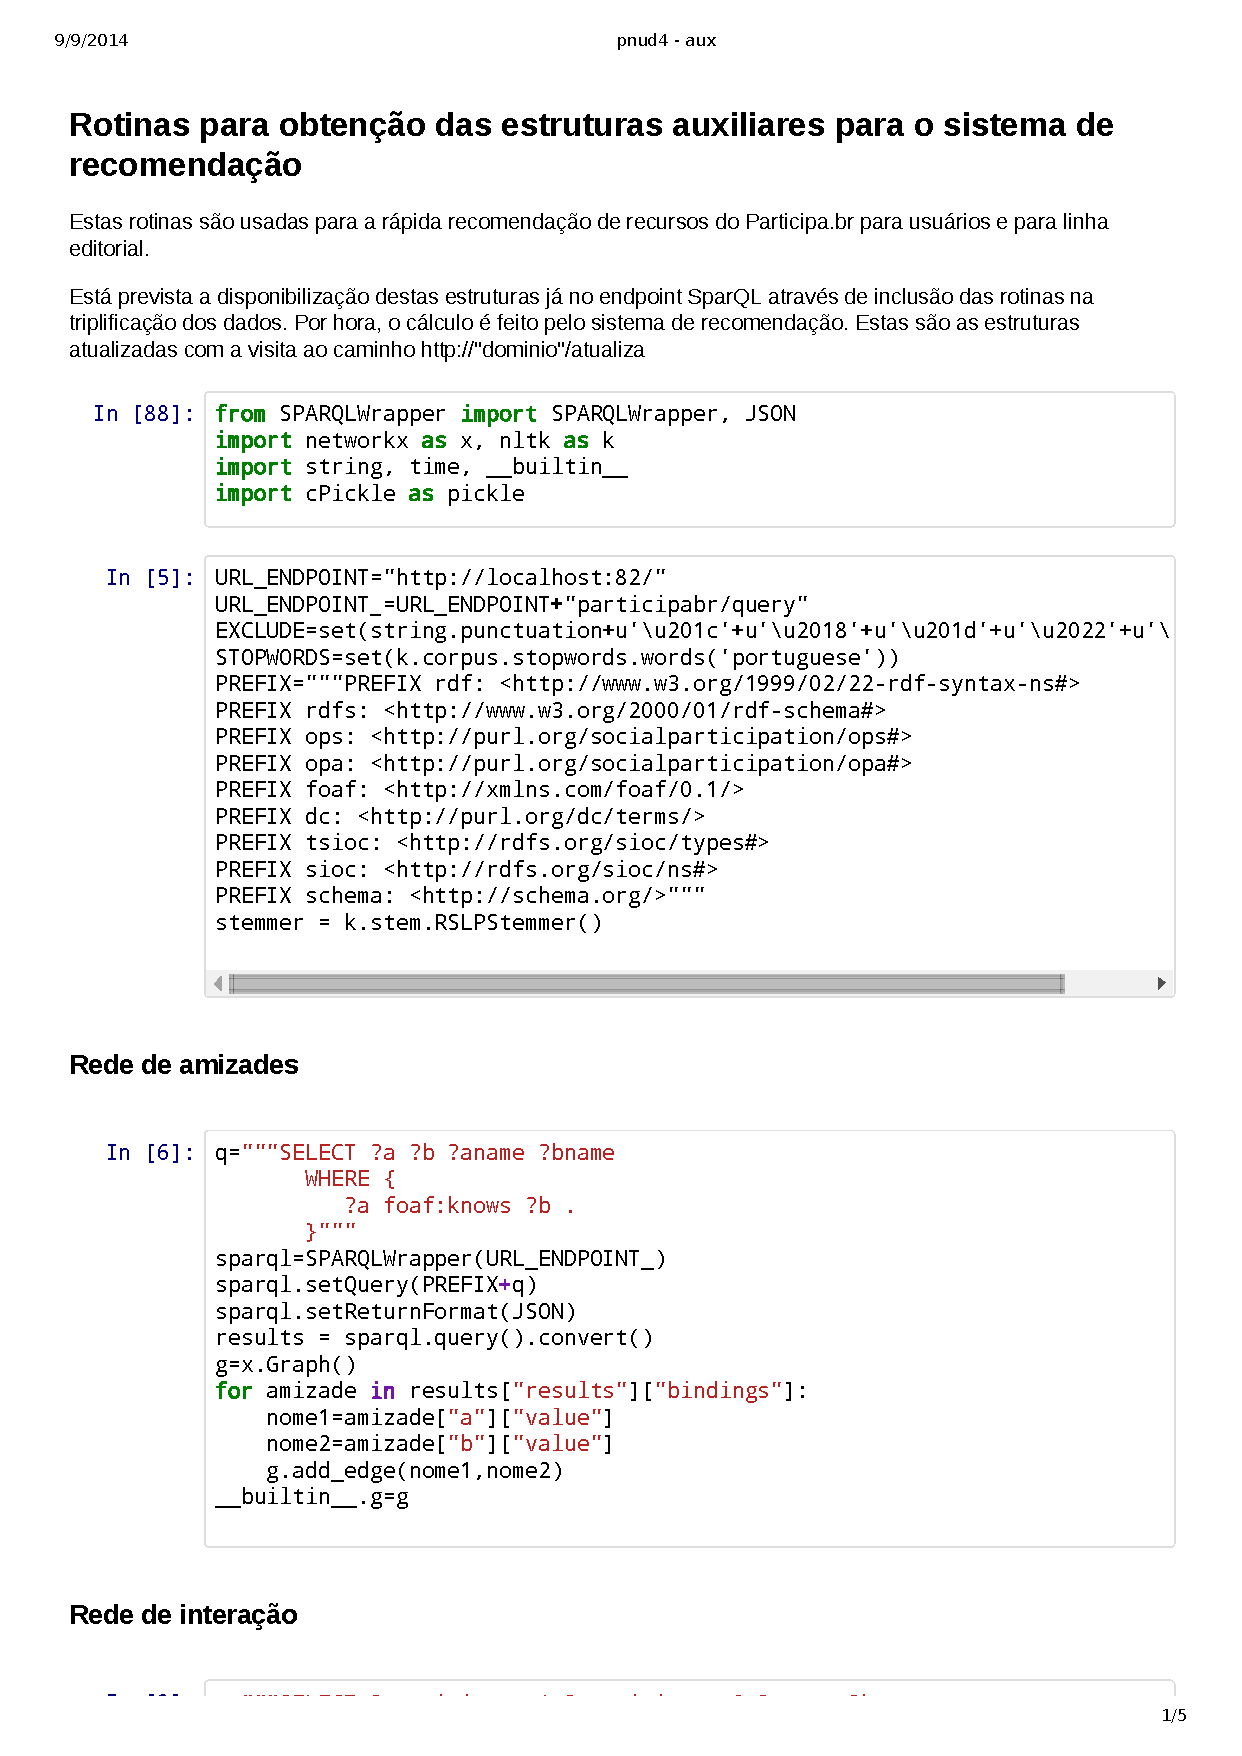
\includepdf[pages=-]{anexos/pnud4aux.pdf}
\subsection{Rotinas para recomendação de recursos}
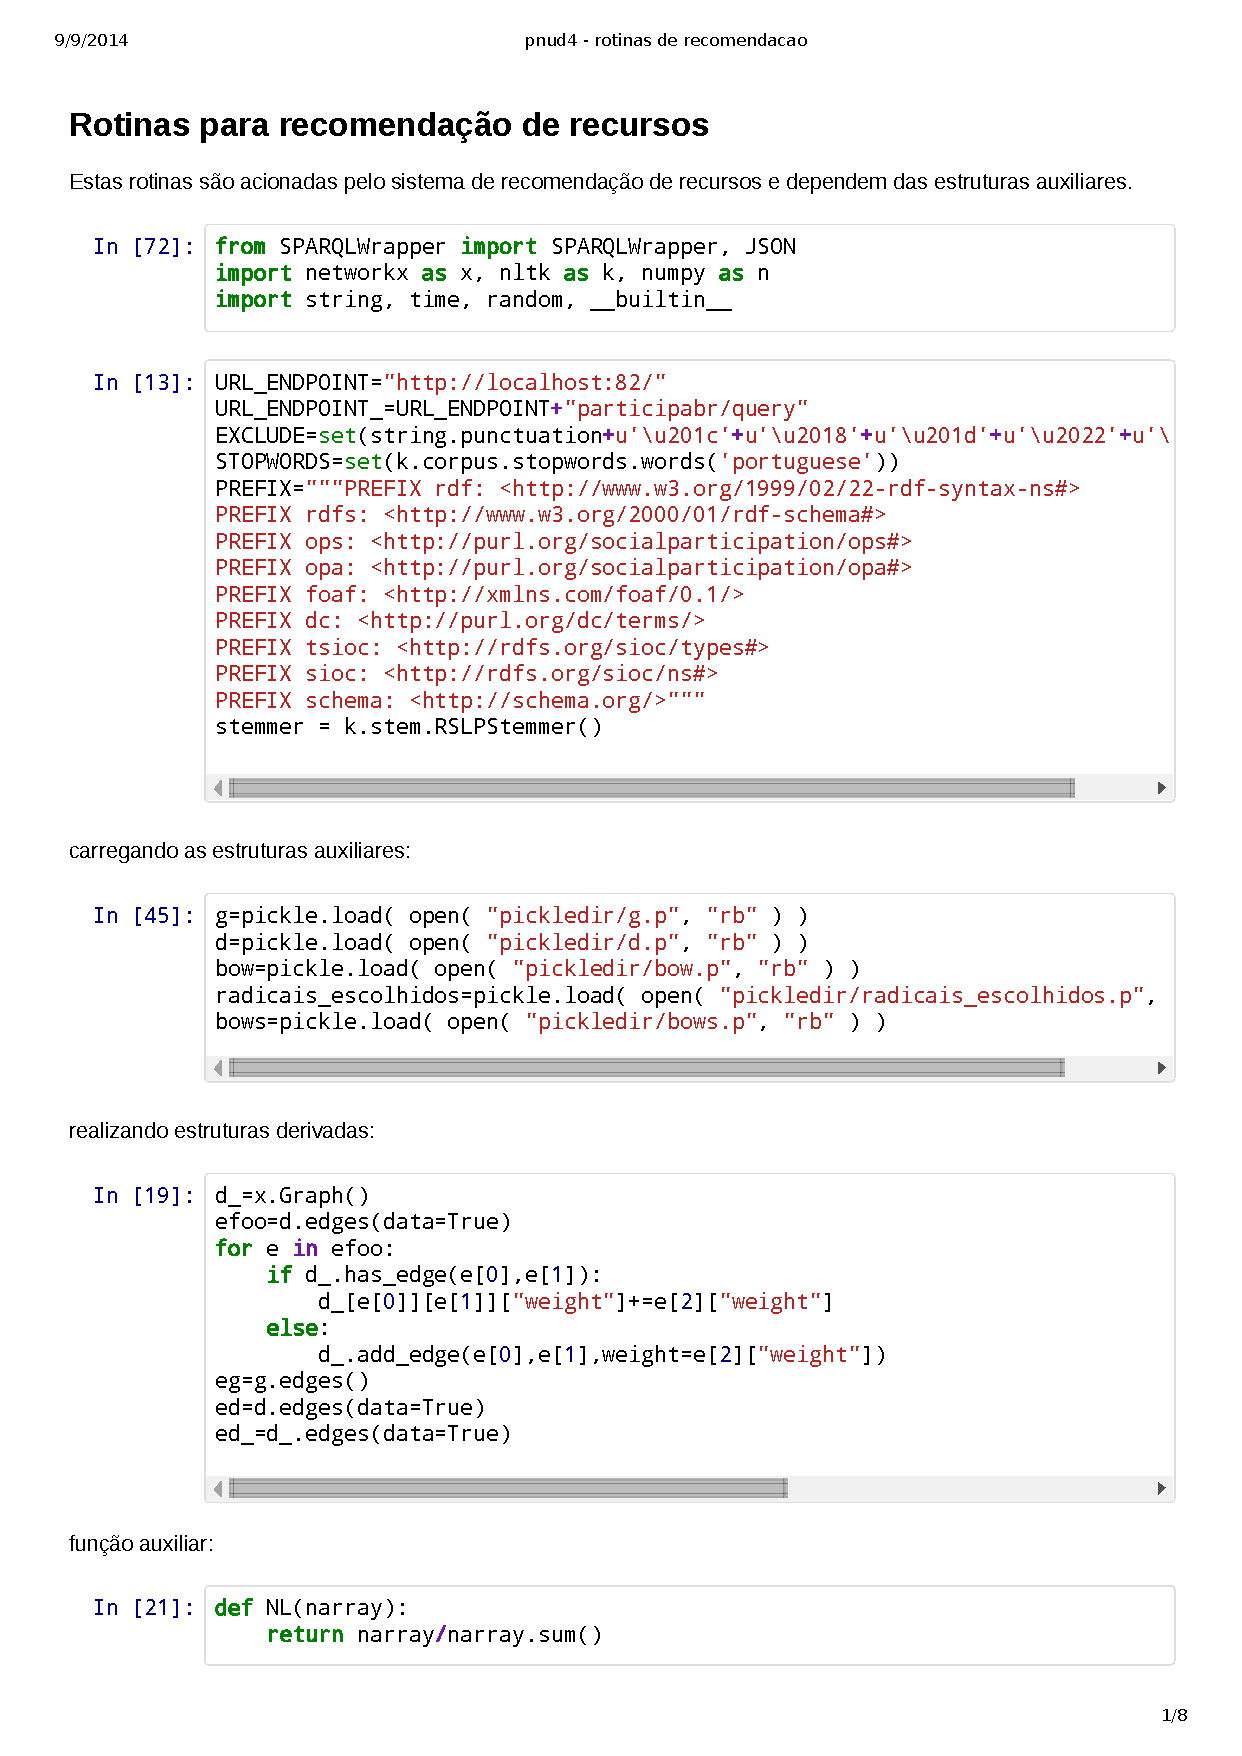
\includepdf[pages=-]{anexos/pnud4rr.pdf}
\section{Parcela dos participantes que produziram texto ou interação}
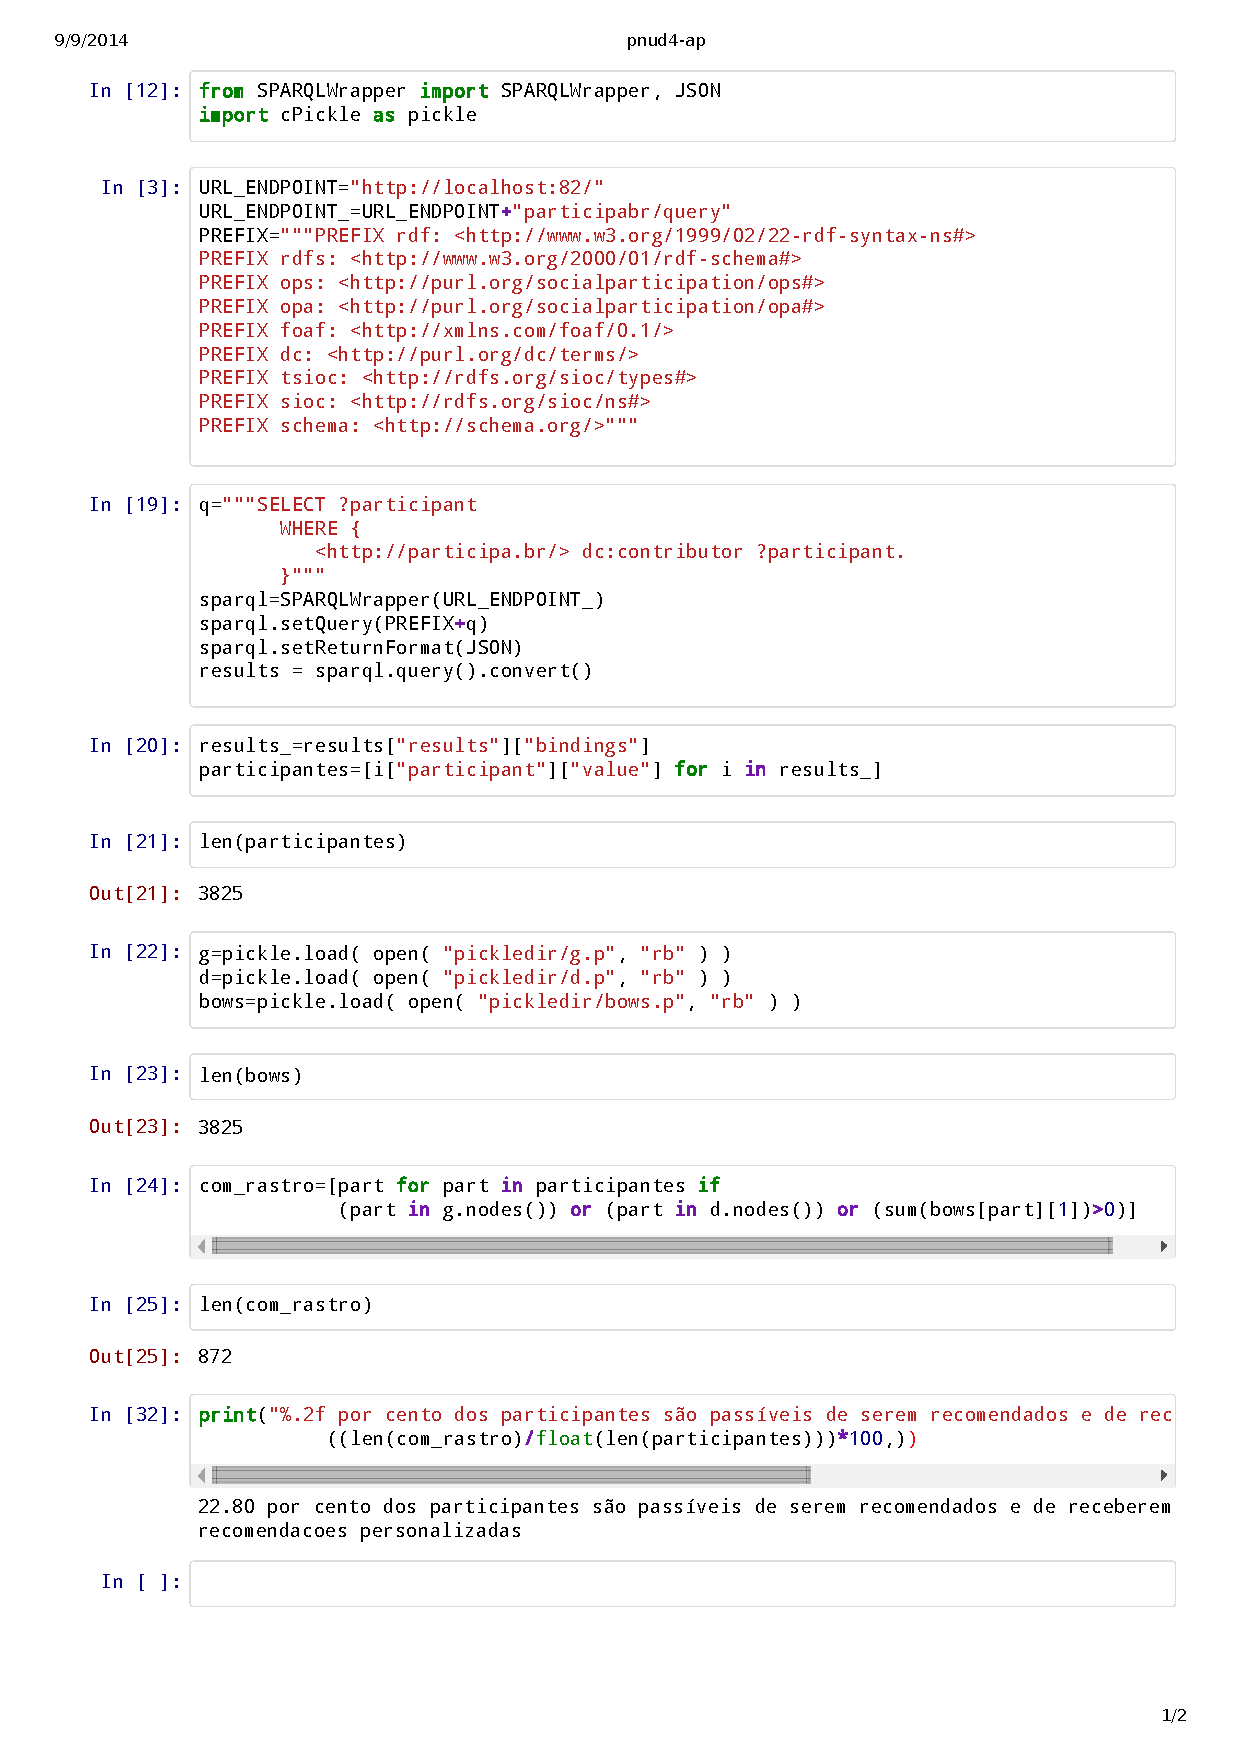
\includepdf[pages=-]{anexos/pnud4-ap.pdf}
\section{Infraestrutura do sistema de recomendações}\label{sec:infra}
A estrutura geral em software e hardware está delineada na subseção~\ref{subsec:hs}
e é tema de todo este documento. Este apêndice descreve os scripts
do sistema de recomendação.

O sistema usufrui do endpoint SparQL para adquirir os dados. O usuário/cliente
do sistema de recomendação acessa URLs via HTTP e recebe JSON, da forma usual.
As rotinas de recomendação em si estão no Apêndice~\ref{sec:algs}. Dada a maturidade
das bibliotecas em Python, a facilidade de desenvolvimento e a capacidade
da comunidade em aproveitar scripts simples na linguagem, todo o sistema de recomendação
está em Python. O servidor HTTP feito em Flask, o acesso ao endpoint SparQL (jena) pelo
SPARQLWrapper, o processamento de linguagem natural em NLTK, os aproveitamentos
das redes complexas em NetworkX. Bibliotecas padrão da linguagem (\emph{builtin} na \emph{Python Standard Library}),
e que estão em uso no sistema de recomendação,
são: json, cPickle, string, random, \_\_builtin\_\_.

O sistema está na pasta flask/ do repositório público~\cite{repoProd4}.
As bibliotecas podem todas serem instaladas via pip e para iniciar o sistema,
basta chamar \texttt{\$ python recomenda.py} ou apontar o apache para a pasta via WSGI.
O sistema levará até 30 minutos para iniciar, pois é necessária a criação das estruturas auxiliares
descritas na seção~\ref{subsec:com}. Este tempo de espera para processar é um dos principais motivadores para incluir estas estruturas nos dados triplificados, disponíveis no endpoint SparQL.

Pode-se considerar os arquivos do sistema de recomendação, disponíveis na pasta flask/, assim:
\begin{itemize}
    \item \texttt{configuracao.py}: variáveis de configuração utilizadas em mais de um arquivo, como a URL do endpoint SparQL, as stopwords consideradas, os caracteres desconsiderados e os prefixos (namespaces) usados para as consultas SparQL. Atualmente \href{https://github.com/ttm/pnud4/blob/master/flask/configuracao.py}{o script} possui menos de 20 linhas de código.
    \item \texttt{auxiliar.py}: rotinas de criação das estruturas auxiliares. Por hora são quatro: 1) redes de amizade e 2) de interação. 3) Histograma de palavras usadas em todo participa.br e 4) por cada usuário. Atualmente \href{https://github.com/ttm/pnud4/blob/master/flask/auxiliar.py}{o script} possui $\approx 150$ linhas de código.
    \item \texttt{rotinasRecomendacao.py}: as rotinas de recomendação de recursos propriamente ditas. Utilizam as estruturas auxiliares e opções dadas pelo usuário/cliente. Retorna recomendações. Atualmente, \href{https://github.com/ttm/pnud4/blob/master/flask/rotinasRecomendacao.py}{o script} possui mais de 350 linhas de código.
    \item \texttt{recomenda.py}: este arquivo levanta o servidor Flask e repassa as opções escritas na URL (método GET) para as rotinas em \texttt{rotinasRecomendacao.py}. Atualmente, \href{https://github.com/ttm/pnud4/blob/master/flask/recomenda.py}{o script} possui menos de 100 linhas de código.
\end{itemize}

\section{Instalação e modificação do sistema de recomendações}\label{sec:inst}
[descrever instalação e possibilidades no heroku. Também do uso do ipython notebook para fomentar inovação]
\section{Propostas de implementações na interface do portal federal de participação social}\label{sec:acr}
Apontar dev do meteor+d3 p dev, processamento e alocação distribuída, além de streaming.
\end{document}
